\documentclass{book}

\usepackage{graphicx}
\usepackage{hyperref}

\title{\textbf{jettl} \\ An Interface-Composition based \\ LabVIEW Actor Model}
\author{Nathan Davis}
\date{\today}

\begin{document}

\maketitle

\tableofcontents

\section{Preface}
\label{sec:preface}

This document is a maximally detailed self-contained document written for LabVIEW developers seeking a proficient understanding of jettl, object-oriented design, and SOLID principles.
To develop not only a strong understanding of jettl, but a strong understanding of modern object-oriented design in LabVIEW by teaching the classical and modernly adopted design patterns along with the SOLID principles.

\section{A Community Effort}
\label{sec:community-effort}

This document is a community effort to create a LabVIEW Actor Model that is interface-composition based.
The goal is to create a design pattern that is easy to use, understand, and extend.
This document is a living document, and contributions are welcome through the
\begin{itemize}
    \item \href{https://discord.gg/tVkvTyBxqa}{jettl Discord Server}
    \item \href{https://github.com/natev51/jettl}{jettl Github Repository}
    \item \href{https://www.google.com/}{jettl User Group(broken link)}
    \item \href{https://www.linkedin.com/in/nathan-davis-0b020a348/}{Personal LinkedIn}
\end{itemize}

Along with reading this document, the model will be best understood with examples that occur in projects.
To show the power of the interface-composition based approach, in particular, examples that are difficult in DQMH, Actor Framework, and other frameworks will be of upmost importance.
This document is meant to be a complete guide to the jettl framework, outlining a starting point for understanding the design philosophy and implementation details.

\section{Introduction}
\label{sec:introduction}

“The fundamental situation is, that we don't know much and some of it's wrong.”
-Carl Hewitt, creator of Actor Model

Package Best Practices:
Reuse code between libraries occurs only by relation (implementation/association/dependency/composition/aggregation) to interfaces.
This is dependency inversion through packages to properly decouple them.

\section{Getting Started}
\label{sec:getting-started}

Before going into any of the internals of jettl, it is important to understand the basic concepts of the framework.

\subsection{Hello World}
\label{subsec:hello-world}

Don't need to send yourself Teardown for Hello World. Just have Teardown method itself at the end of the Hello World Msg.
Since this message is being sent to yourself, the message will be in the actors library and marked private, so other actors cannot implement this message.

\begin{figure}
    \centering
    \includegraphics[width=0.8\textwidth]{figures/Hello-World}
    \caption{This image shows the hello world example.}
    \label{fig:hello-world}
\end{figure}

\section{Class Hierarchy}
\label{sec:class-hierarchy}

\begin{figure}[ht]
    \centering
    \includegraphics[width=0.8\textwidth]{figures/class-hierarchy}
    \caption{jettl Class Hierarchy.}
    \label{fig:jettl-class-hierarchy}
\end{figure}

Fig~\ref{fig:jettl-class-hierarchy} shows the class hierarchy of jettl.

Actors are responsible for their own references. In particular:
\begin{itemize}
    \item Queue: Obtains and releases its own references.
    \item Event: Creates, Registers, Unregisters, and Destroys its own references.
\end{itemize}

\begin{figure}
    \centering
    \includegraphics[]{figures/project-screenshot}
    \caption{This image shows the jettl project in LabVIEW.
        The project contains the jettl library, which contains the Base Queue and Base Event classes, along with the Queue Mailbox class.}
    \label{fig:project-screenshot}
\end{figure}

\section{Last Ack}
\label{sec:last-ack}

\begin{figure}
    \centering
    \includegraphics[width=\textwidth]{figures/queue-mailbox-duplicates}
    \caption{There exist duplicates in the Queue Mailbox and respective Base Queue jettl and Base Event jettl because the Last Ack message uses the alias of the closed down actor and this cannot be in the Queue Mailbox DVR since the DVR will have already been released.
        So there exists duplicates for the Self Queue Alias, Self Queue, Self Event Alias, and Self Event so that the Last Ack can still access these, even after the DVRs have been released.}
    \label{fig:queue-mailbox-duplicates}
\end{figure}




\section{Unit Testing}
\label{sec:unit-testing}

With the Queue interface, this model is interface-composition based with the decorator Pattern, so unit testing is built in by decorating the Base Queue class with other classes that implement the Queue interface or Event interface.
In effect, instead of wrapping the Base Queue with your Develop class, you can wrap the Base Queue with a Debug Queue class, which is wrapped with your developed class.
This occurs since these all inherit from the same Queue interface.

\begin{figure}
    \centering
    \includegraphics[width=0.4\textwidth]{figures/wrapping-idea}
    \caption{This image shows the Queue Base Debug class and is a wrapper around the Queue Base class for debugging purposes.}
    \label{fig:wrapping-idea}
\end{figure}

One can see immediately that an infinite number of classes can be decorated, leading to a powerful feature of the interface-composition based decorator pattern.

\section{Tools}
\label{sec:tools}

\section{Debugging}
\label{sec:debugging}

\subsection{Displaying Method Execution}
\label{subsec:displaying-method-execution}

What a log for which methods are executed, instead of the dialog popups

Two project conditional blocks:
\begin{enumerate}
    \item Occurs in all methods(?)
    \item Occurs only in message specific methods
\end{enumerate}

These conditionals occur in both Base Queue and Base Event classes.
If either conditional is true, debug panel that displays the names of actors (columns), along with timestamps (rows) of when methods (data) are executed.
Think discrete time water fall display.


\section{Examples}
\label{sec:examples}

\subsection{Nested Actors}
\label{subsec:nested-actors}

\href{https://youtu.be/N6X9KyJJ-D4?feature=shared}{2018 NIWeek Allen C Smith Efficient Actor Framework Development}
25:58
Teardown vs Orderly Teardown:
Allen wanted a “Stop Nested Actors Msg”, SLM against.
There include two methods: Event Nested Teardown.vi and Queue Nested Teardown.vi.
These two methods are used to teardown the respective nested actors.

\subsection{Sending Event Message}
\label{subsec:sending-event-message}

Button press sends message to Self (queue actor).
Queue actor internally sends a string indicator Event which occurs in event loop.


\section{Design Patterns}
\label{sec:design-patterns}

\subsection{Strategy Pattern}
\label{subsec:strategy-pattern}

\subsection{State Pattern}
\label{subsec:state-pattern}

\noindent Context:

\quad Method.vi (just a wrapper for Method.vi “State”).\footnote{Best Practice: use this Method.vi in other methods, rather than the Method.vi “State” itself}

\noindent State.lvclass (interface):

\quad Concrete State.lvclass

\quad Method.vi “State”

\subsubsection{State Pattern Privacy}
\label{subsubsec:state-pattern-privacy}

Context classes should be private, since only interface objects should be composed into a class.
Dependency Inversion Principle.
Since the context class is private to the library it is in (and the State Interface with its concrete state classes), public static dispatch methods can be used in the context class AND concrete state classes without worrying that they'll be used outside the library since the context class is private.

\subsection{Decorator Pattern}
\label{subsec:decorator-pattern}

\subsection{Memento Pattern}
\label{subsec:memento-pattern}

When saving the state of an actor, the Memento Pattern is used.
Instead of sending the entire actor state in Actor Last Ack Msg, there should be another dedicated message that sends the actors state to the calling actor.
This has not been done, but it is a good idea to implement this in the future.

Memento, actors shouldn't know about each other, so if the state of a nested is to be saved, then there is a separate message for this since last ack shouldn't know about this.
Rather, this specialty message couples with last ack if the developer wants this functionality.


\subsection{Factory Pattern}
\label{subsec:factory-pattern}

The Factory Pattern is used to create instances of actors without specifying the exact class of the actor that will be created.
This allows for greater modularity in the actor design.
Easy Factory pattern integration with Queue and Event Interfaces for plug and play architectures.


\subsection{Observer Pattern}
\label{subsec:observer-pattern}

Actors references cannot be passed between actors or helper loops.
They are intentionally abstracted away from the developer.
Now, because helper loops are async and own their own references.
Their references can be passed around the actor tree.
This provides a modular way of sharing async references, following the observer pattern.

\begin{figure}
    \centering
    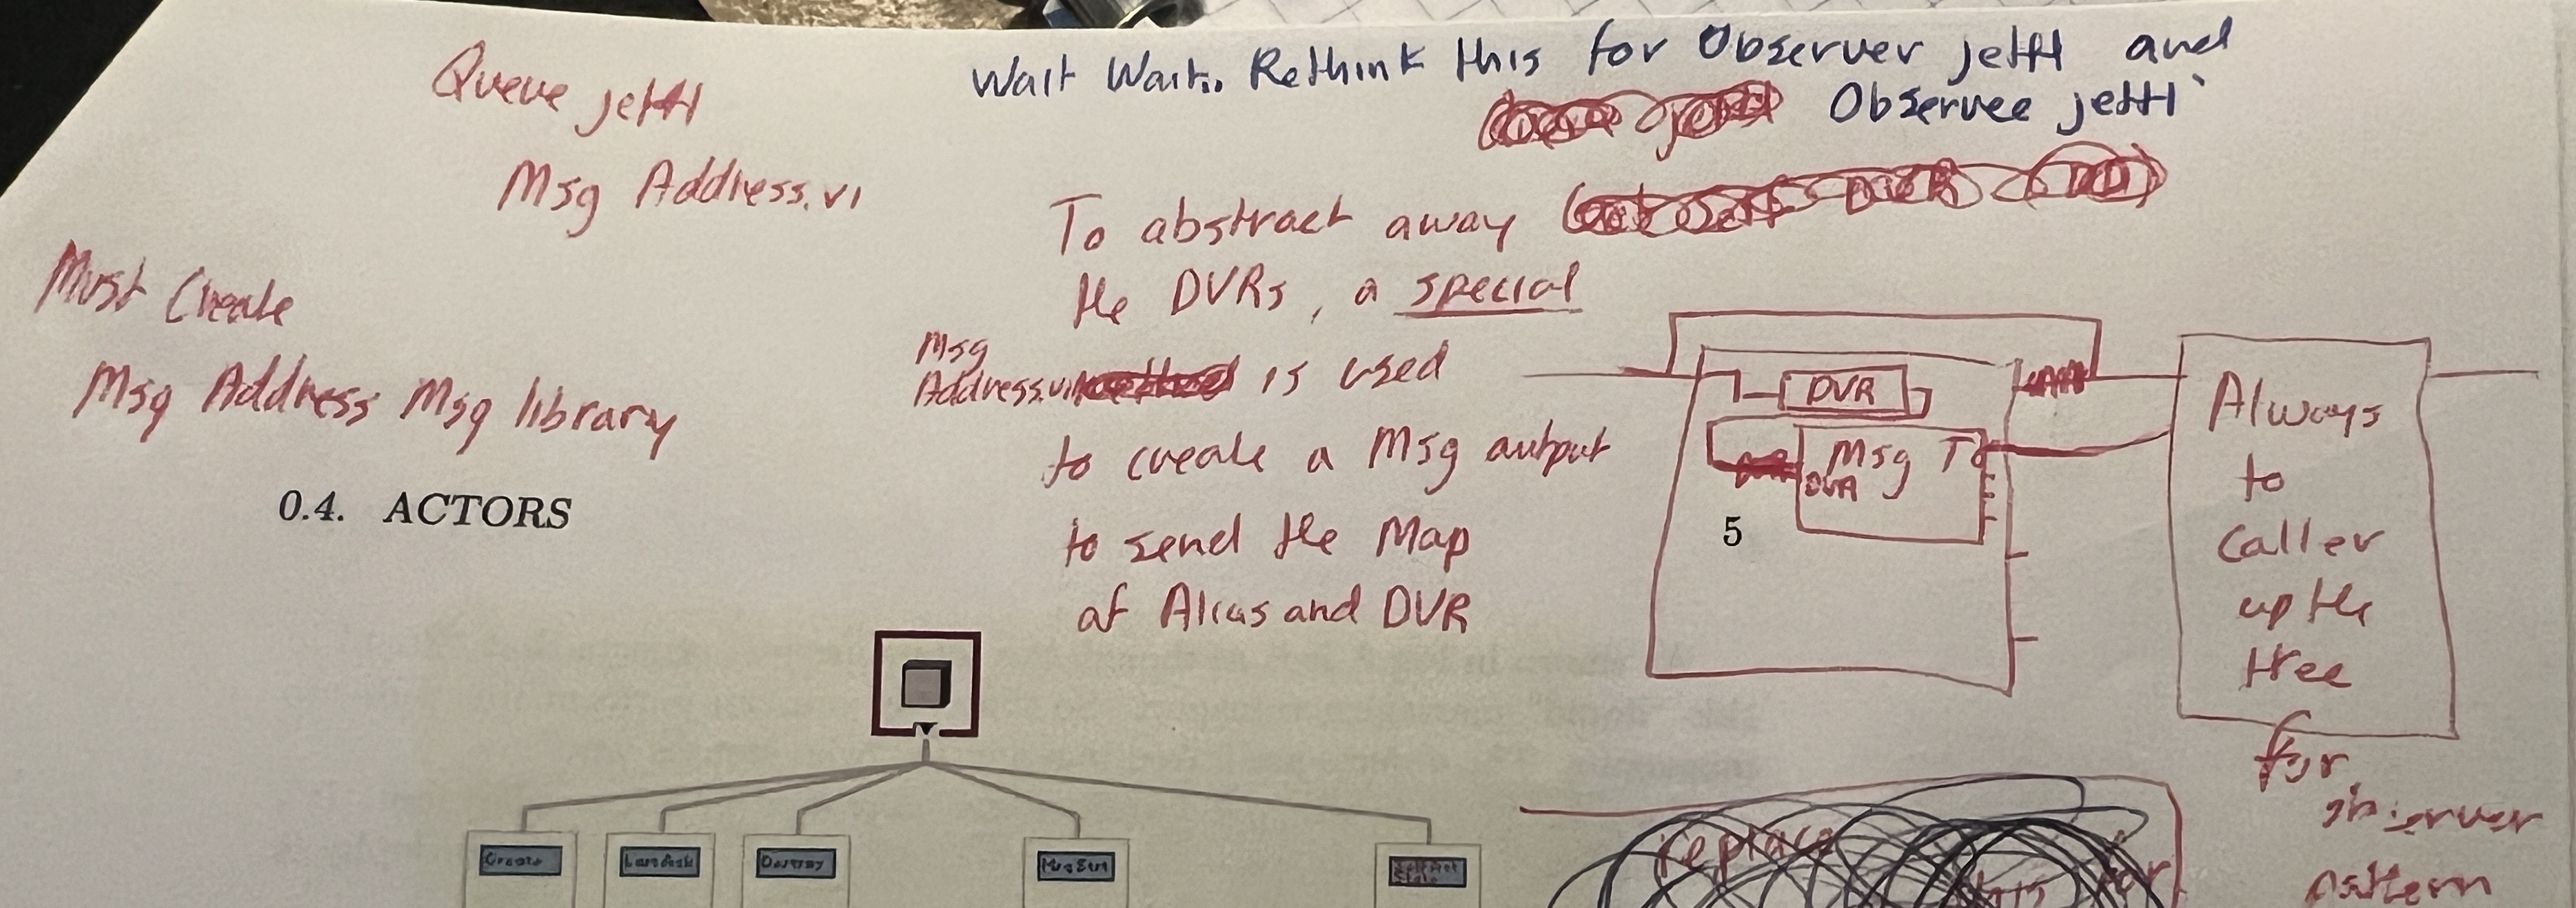
\includegraphics[width=\textwidth]{figures/Observer-idea}
    \caption{This image shows the observer pattern in jettl. The observer pattern is used to send messages across the actor tree.}
    \label{fig:observer-idea}
\end{figure}

An actor is NOT connected to the actor that creates it, but does have its immediate references to send messages.
Rather, this actor exists on its own in the “liquid” message transport.
The overall “application” has access to the actor's reference (unique message address), defined from the DVR in the Base classes private data.

\begin{figure}[ht]
    \centering
    \includegraphics[width=0.8\textwidth]{figures/labview_dmitry_message _transport}
    \caption{LabVIEW Actor Framework Message Transport.}
    \label{fig:message-transport}
\end{figure}

As shown in Fig~\ref{fig:message-transport}, it is as though the actors are just objects that “float” in this “liquid” messaging transport.
So that way you can perform this pub-sub messaging.
The objects are linked together by “who creates who”.

Same as with the pub-sub pattern, everything is a publisher-subscriber.
It's just that most relationships are just one way.
Same with Git, the philosophy is that all branches are created equal.

\section{Event Actors}
\label{sec:event-actors}

This is to declutter the actor by offloading certain tasks such as panel display or subprocesses that do not require an additional actor to be created.
Since the Event Actors are not dependent on the Queue Actor, we can unit test an Event Actor.

Event Actors are created using Event Create.vi, where the wired in object optionally has a method for bundling in the necessary private data.

\subsection{Event Actor Best Practices}
\label{subsec:event-actor-best-practices}

References should not change after they are created.

\subsection{Event Actor Benefits}
\label{subsec:event-actor-benefits}

Event are designed to be reusable and modular.
Event Actors are not tied to the Queue Actor that creates them.
Furthermore, Queue Actors should not depend on Event Actors.

These can be orphan processes i.e. they are not tied to the lifetime of the actor that creates them.

\section{Event Loop}
\label{sec:event-loop}

It is safe to send messages to the Caller, Self, AND Nested Actors.
Nested actors will have the correct Msg Queue since they're updated when a Queue Nested is created in the Queue Actor.
Check details outlined in the Queue Actor.vi within jettl Queue Actor.lvclass.

This method works for all types of Event Actors.
In particular, ones with shown panels since the window appearance can be changed between DD methods.

Philosophy:
An actor messaging should be running for the entirety of the actor.
That means if you want to change an actors panel, some other entity should be changing its panel for the actor.
This separates the concerns from the actor and the panel.

\subsection{Window and Subpanel Event Actors}
\label{subsec:panels}

\begin{figure}[ht]
    \centering
    \includegraphics[width=0.8\textwidth]{figures/justACS_ui_events}
    \caption{This image shows the UI events in LabVIEW.}
    \label{fig:justacs-ui-events}
\end{figure}

Split the events as controls and indicators as shown in Fig~\ref{fig:justacs-ui-events}.

\subsection{Synchronous Event Actor}
\label{subsec:synchronous-event-actor}

Since Queue Actors should always be ready to dequeue messages, it should not wait on a response.
Rather, the Queue Actor should create the Synchronous Event Actor.
When the Event Actor is waiting for response, that's okay since when the event actor is waiting, it is also ready to teardown whenever since it is always waiting for an event.

\subsection{Event(?) Observer}
\label{subsec:event-observer}

A Queue Actor has in its project an Event Actor that another Actor can create. And here can send its Event Actor Ref to the Libraries Queue Actor to pump messages across the tree.
For reusability, a Queue Actor has in its project the Event Actor that another Actor can create.
And here can send its Event Actor Ref to the Libraries Queue Actor to pump messages across the tree.

\begin{itemize}
    \item NIAF: 2-Dimensional tree hierarchy
    \item Base jettl: 3-Dimensional hierarchy
\end{itemize}

In Base Queue, a tree hierarchy of Queue Actors (follows 2-dimensional NIAF messaging scheme) and a single layer tree hierarchy of Event Actors for a given Queue Actor.
The 3-Dimensional aspect comes from Event Actors being able to share their references with other Queue Actors and/or Event Actors.
This allows these latter Actors to send events to the respective Event Actor who has shared their reference.
This “messaging across the tree” in three dimensions can occur giving rise to a type of observer pattern (publisher/subscriber).

\section{Notifier Actors}
\label{sec:notifier-actors}

Notifier Actors are created using Notifier Create.vi, where the wired in object optionally has a method for bundling in the necessary private data.

\subsection{Notifier Periodic}
\label{subsec:notifier-periodic}

This could be an event actor, but notifiers work well with timing.
If it was an event actor, then the event actor would have to wait for the next event to occur via the timeout case in the event loop.
But there would be interruptions in the event loop, which would cause the event actor to not be able to send messages at the correct time.

Private Data:
\begin{itemize}
    \item Iteration (0 = infinite) (U32)
    \item Period (ms) (default 1000) (U32?) (cannot = 0)
    \item Initial Wait (ms) (default 0) (U32?) (cannot = 0)
\end{itemize}

Along with the Stage Pattern used in the Base Notifier.lvclass, State Pattern can be used in the Notifier Periodic.lvclass such as
\begin{itemize}
    \item Idle State
    \item Running State
\end{itemize}

\section{Messaging}
\label{sec:messaging}

Messages do not have error wires since errors are handled internally in the Base classes.
This is because the Base classes have an error cluster in their private data.

These messages follow the Interface Segregation Principle (ISP) by having one method in the messages interface.

All messages come from an interface and follow ISP where one message belongs to one interface.
If there is a naming issue, that is a good thing.
It means in the dependencies, you should be packaging modules so you don't run into naming issues.


All messages are interface messages.
Note, they do not need to be implemented.

Actor messages error on generation of message.
Error when creating a message and wiring in the interface object as an input, the message scripting doesn't know how to differentiate the class input and the parameter input.

\subsection{Private Messages}
\label{subsec:private-messages}

Private messages that aren't exposed to external callers: Library access scope.
To conform to this, the Last Ack messages should be private messages to the Queue Base class.
This is because the Last Ack messages are not intended to be used by external callers.
Further, this should also be done for the Update Queue Nested message. This should not be used by external callers, but rather only by the Event Base class.

\subsection{Messages Up and Down the Tree}
\label{subsec:messages-up-and-down-tree}

When messages are sent up the queue tree, followed by being sent down the tree, the developer could consider using event actors to message across the tree.
This is a direct use case for using an Event Actor.
Sharing the event actor reference to the necessary Queue Actors or Event Actors for direct communication.
This is the power of Event Actors.
Gives rise to the Observer (Pub-Sub) Pattern, sending NOT Msgs, but Events across the tree.

\subsection{Messages with Type Definitions}
\label{subsec:messages-with-type-definitions}

Type definitions as inputs SHOULD be in the library, not the class they're implemented in.
This is fundamentally an exercise in dependency inversion.

Cluster message with type def inside of the library.
Good practice to put the type def here and NOT in the class that implements the message.
This takes care of otherwise awful circular dependencies.

\subsection{Scripting}
\label{subsec:scripting}

Tips:
Go through and replace all the Opens and Traverse with the hidden gem.
User groups for the scripting (quick drop, right click, etc.).

\subsubsection{Right Click Message Creation}


\section{TODO}
\label{sec:todo}

In the DD methods, because they are not required to be overridden, have functionality within them that calls the Self Actor method (some kind of checking mechanism?).

Actor interface methods (all implemented with default functionality) to have the *new* (Actor Interface) Read Actor DD method that reads from the Dev Actor the Self Actor class and performs that interface function, then bundles back in with the Setup method.

Do this for all for the default behavior.

Note this is breaking the contract for interface DD methods not needing to be overridden.

Instead of the Setup method, create a new Actor Write method which ONLY Writes to the Actor. This can also be put inside the Setup method as a first step, the setup code follows after

State Enter Core and State Exit Core are NOT check marked.
That way the developer does not need to override, just to have no functionality anyway.
Read State and Write State do because they'll have functionality.

\section{Errors}
\label{sec:errors}

In frameworks, errors are fundamental to the program's operation. They are not just incidental issues but rather integral to the design and flow of the application.
jettl has an error object in the private data of the jettl object. At the end of the method, the error object is unbundled and checked for errors before teardown.

Error philosophy: Errors occur ONLY from unexpected events.
For example, the error case in Msg.vi: in the case structure, a custom error saying that a message could not be executed occurs when 'message name' occurs for 'actor name'. This is unexpected behavior since this SHOULD be known at edit time. This is a legit error.

'That was handled, or I wouldn't have been called' - SLM (\href{https://www.youtube.com/watch?v=00TZxeyt8_A}{The Errors of our Ways | Stephen Loftus-Mercer GDevCon N.A. 2021: 52:08})

Wouldn't this make the API more beautiful and easy to understand? Having just the object wire come out of the method, and ONLY the object wire coming out of the method?
I suppose, adopting the OO paradigm.
Instead of having the error cluster inside the objects class data.
Instead, it's a dedicated “error cluster” shared for every single object in use.
Encourages data flow since unbundling of errors will always occur.
It's a step in the right direction having no “error input” for methods.
Now it's time to get rid of the error out.
It's almost like branching an objects wire, in a way. There should only be one thing coming out of a method.

\section{Example}
\label{sec:example}

\subsection{Dev Actor}
\label{subsec:dev-actor}

Merge Error and Override Error are decorators used.
Otherwise, the other DD methods are trivial and only used once.


\section{Creation}
\label{sec:creation}

\begin{figure}
    \centering
    \includegraphics[width=0.8\textwidth]{figures/Creation}
    \caption{This image shows the creation of Base Actors.}
    \label{fig:creation}
\end{figure}

Queue Actor
\begin{itemize}
    \item Has One Caller Queue Actor
    \item Is a Nested Queue Actor of Queue Actor
    \item Is a Self Queue Actor
\end{itemize}

Event Actor
\begin{itemize}
    \item Has One Caller Queue Actor
    \item Is a Nested Event Actor of Queue Actor
    \item Is a Self Event Actor
\end{itemize}

Framework constraint:
A Queue Actor can create both Queue Actors and Event Actors whereas an Event Actor cannot create either.
The Event Actor can queue itself either Queue Create or Event Create messages, but this goes to the Queue Actor to handle these.
The handling does not occur in the Event Actor since the Event Actor cannot create.

A future question: Should Launch.vi exist outside the Queue Base class?
If it does, then Queue Base can be marked as a private class, and the Launch.vi can be public.

Only Queue Actors can create Queue Actors and Event Actors.
Event actors cannot create either.
Further, because of these rules, only queue actors can receive the Last Ack from Nesteds.
This is respectively the Queue Last Ack and Event Last Ack.
Event Actors cannot receive either Last Ack.
These Last Ack messages are not used by the developer.
These occur in the framework itself, though functionality can be wrapped in the developed queue actor.


\section{PPL Support}
\label{sec:ppl-support}

Note that jettl is designed with PPLs in mind!
This is because
\begin{itemize}
    \item jettl comes as a single library, so it can be packed into a PPL without external dependencies
    \item To change a class to use the PPL version of jettl is to change the
          \begin{itemize}
              \item implemented interface to the PPL one and
              \item compose in the PPL Interface.
          \end{itemize}
    \item jettl does not include:
          \begin{itemize}
              \item xnodes
              \item malleable VIs
          \end{itemize}
          xnodes and malleable VIs cause build issues with PPLs, they do not exist in jettl.
\end{itemize}

For more information on PPLs, Darren Nattinger and Derrick Bommarito have excellent content:
\begin{itemize}
    \item \href{https://forums.ni.com/t5/Community-Documents/Debugging-Symptoms-Packed-Project-Library-PPL-Dependencies/ta-p/4107786}{Debugging Symptoms - Packed Project Library PPL Dependencies - Searching for Dependencies Dialog When Running Executable}
    \item \href{https://forums.ni.com/t5/LabVIEW/PPL-Namespaced-Dependencies-Strategy-Design-Discussion/td-p/4276248}{PPL Namespaced Dependencies - Strategy/Design Discussion - Development Issues}
    \item \href{https://www.youtube.com/watch?v=HKcEYkksW_o}{LUDICROUS ways to Fix Broken LabVIEW Code with Darren Nattinger | GDevConNA 2022}
\end{itemize}

\section{Opinionated Design Choices}
\label{sec:opinionated-design-choices}

Virtual folders are not saved on disc.
These are only convenience in the LabVIEW project.

\subsection{Accessors}
\label{subsec:accessors}

Since class inheritance is not used, accessors **are not** used very often (aside from tightly coupled classes such as State Pattern).
This is especially true with Actors.
Actors are self-contained and will rarely allow other classes to use its attributes.

\subsection{Color Scheme}
\label{subsec:color-scheme}

"Look down at the green grass, look up to the blue sky, and look further to the purple galaxy."
\begin{itemize}
    \item Purple Library: RGB (166,153,182)
    \item Blue Interface: RGB (104,136,190)
    \item Green Class: RGB (110,149,108)
\end{itemize}

\subsection{Icons}
\label{subsec:icons}

\begin{itemize}
    \item Shows interface / class name.
    \item Color of banner indicates if a library/interface/class container.
    \item Text of method name.
    \item Color of method name indicates access scope of method/control.
\end{itemize}

\subsection{Access Scope}
\label{subsec:access-scope}

Only public and private.
Interfaces, classes, and methods have text in the icon/banner that are black for public and red for private.
Private data text icon is red for class private data since inherently private.

Emphasis is put on encapsulated classes are classes (maybe container libraries) marked private.
Class encapsulation. Any class should be marked as private to the library containing them.
That way, it is not encouraged to use the classes in other projects, leading to use of dependency inversion.
Or, stipulation, classes that are held in libraries, the library should be marked as private.
Red private banner, even if the class is public but in a privately marked library
This occurs when the classes are tightly coupled, such as with the state pattern.

Rules:
\begin{itemize}
    \item Nested Libraries should be marked private, otherwise, put the nested library outside the containing library
    \item Classes should be within at least one library
    \item To promote dependency inversion: A class should be marked private, but only public IFF within a private nested library. This keeps from others from using the class in the containing library, BUT breaks true dependency since other classes can use the class in the containing library
    \item Interfaces and classes must be contained in at least one library
\end{itemize}

To promote dependency inversion:
A class can be marked public IFF within a private nested library
This keeps from others from using the class in the containing library, BUT breaks true dependency since other classes can use the class in the containing library.

\subsection{Errors}
\label{subsec:errors}

Errors are built into jettl.
For every actor being wrapped, there is an error cluster within their private data.
The errors are abstracted away from you, but if there does exist an error you may handle it in the Handle.vi override.

Except the error that could potentially occur at the end of Queue Actor.vi and Event Actor.vi, no error goes unrecognized.
Why are there are so many error case structures?
All methods in Base jettl are assumed to run unconditionally when they are called.
Also, no serialization of errors.
Instead, it is serialization of the object wire since internally, the class on the interface object in the private data has an error cluster.
The merge errors method (which internally has the Is Error.vi), dictating if Base jettl should enter the respective Error State.

Abandoning Data type IO Serialization:
An indication that the data in the data type will *potentially* be manipulated is when a data type is being passed in and out through a method.
Unless a data type can be manipulated in an Interface/Subclass/Subinterface, then the data type should not have an output.

If a method must be serialized, embrace the flat sequence structure / error case structure.
DO NOT pass a data type from the input to the output of the method for the *sole purpose* of serialization.
Understand that other developers will not know your intent and will assume that the data in the datatype will *potentially* be manipulated.
Not wiring the outputs gets rid of this thinking entirely for better readability.
Further, do not serialize by using an error cluster input and output.
This provides difficulty for readability since the developer does not know if the error is being manipulated by the method.

No error goes unnoticed in the framework, everything is reported (except for releasing references).

Error Serialization:
The traditional error input is not allowed.
A method should execute unconditionally.


\section{Queue Mailbox}
\label{sec:queue-mailbox}

Ideally speaking, there would be a Mailbox interface that Queue Mailbox implements.
But since the interface checkbox is checked and cannot be changed: "Data Value References - Restrictions On New and Delete: Enabled: Restrict references of this class type to member VI's of this class", that means that Interfaces cannot be a DVR.
Further, this immediately voids any dependency inversion since an object in a DVR cannot change its object, by definition such as what dependency inversion does.
Therefore, the Queue Mailbox in the Queue Mailbox library cannot be marked private, allowing other classes in the jettl library have access to it via the DVR.
This really isn't a problem though since the Queue Mailbox library is marked private, so nothing outside the jettl can use this class and DVR methods, encapsulating the DVR, as intended by jettl.

This should be where the new queue nested should be sent via event to update the Queue Nested in Event Actor.
Yes, it is not instant, but gives the Event Actor(s) the reference so they can send messages to this newly created Queue Actor.
Beware, here with these being async processes, temporal issue may arise.

\section{TO ORGANIZE}

\begin{figure}
    \centering
    \includegraphics[width=\textwidth]{figures/event-loop}
    \caption{Event Loop. This shows the event loop in jettl.}
    \label{fig:event-loop}
\end{figure}

\begin{figure}
    \centering
    \includegraphics[]{figures/jettl-palette}
    \caption{jettl palette.}
    \label{fig:jettl-palette}
\end{figure}

\begin{figure}
    \centering
    \includegraphics[]{figures/jettl-palette-msg}
    \caption{jettl message palette.}
    \label{fig:jettl-palette-msg}
\end{figure}

\begin{figure}
    \centering
    \includegraphics[width=\textwidth]{figures/class-hierarchy}
    \caption{Class Hierarchy. This shows the class hierarchy in jettl.}
    \label{fig:class-hierarchy}
\end{figure}

\begin{figure}
    \centering
    \includegraphics[width=\textwidth]{figures/queue-actor-method}
    \caption{Queue Actor Method. This shows the method for the Queue Actor in jettl.}
    \label{fig:queue-actor-method}
\end{figure}

\begin{figure}
    \centering
    \includegraphics[width=\textwidth]{figures/event-actor-method}
    \caption{Event Actor Method. This shows the method for the Event Actor in jettl.}
    \label{fig:event-actor-method}
\end{figure}

\begin{figure}
    \centering
    \includegraphics[width=\textwidth]{figures/alternate-start-async}
    \caption{Alternate Start Async. This shows the alternate start async in jettl. Note this is outdated naming, but the functionality is still the same.}
    \label{fig:alternate-start-async}
\end{figure}

\section{Assembler}
\label{sec:assembler}

Previous idea to *maybe* get back to..
Mediator pattern is data flow friendly and DOES NOT cause memory leaks since a created Actor only occurs once at a time, through the mediator.
And can only shut down if the mediator says that the Actor should shut down.
The mediator knows who has whose reference to send messages.
This helps establish the observer pattern too.
No deadlocks can occur since the mediator operates one by one.
It is the all-knowing for the program, only forwarding messages to references that the message is intended for.
An actor ever only knows about the mediator.

Kind of the same framework you currently have.. just that the messages interact with a mediator that then (since it has references to everything) sends the message to the necessary actor.
Note the Self Actor still has references to its Creator, Self, and Created.. it’s just that the mediator ALSO knows who has these references and easily sends the message to those who have the reference that the message is going to has.
This provides well for the observer pattern i.e. publisher and subscriber.
There are effectively two places references are saved: Mediator and Self Actor.
The Mediator always has the references and shares the necessary duplicates of references that pertain to the Self Actor since these are references to identify the Actor and how the mediator should allow the actor to interact with other actors (though, remember, the Actor doesn't know other actors exist.. only that there is a mediator).
Further, the mediator knows which methods are messages of the actor.
This is known at compile time since messages are all through interfaces, allowing the mediator to know which messages the actor can execute by checking which interfaces the actor implements.
This check happens in the mediator, not in the actor.
This can be a set of strings relating to the method name?, so upon creation of an actor (by the mediator), the mediator holds the reference to the actor and a *set* of method names that are tied to messages.

Just thinking out loud, here is a concrete component that basically handles the business logic of the system with other sub business logic components that are more specialized / reusable. This can be thought of as some top level actor.

Multiple application instances Idea:
Application mediator that is between all.
Or there is always a double layer of mediators?
Where the top layer facilitates what the lower mediator does.. and when there is another application instance (which has its two mediators), the top mediators of both communicate to each other.
The top mediators know about each other's references, so they can communicate with each other.

If two applications are talking with each other, there now exist two mediators.
An idea for this: there is again a mediator that is *above?* these two mediators?

\begin{figure}
    \centering
    \includegraphics[width=0.8\textwidth]{figures/assembler-hierarchy}
    \caption{Assembler. This shows the assembler in jettl.}
    \label{fig:assembler-hierarchy}
\end{figure}

Assembler strictly for passing references to other Queue jettls for the Observer Pattern.

Queue jettl cannot create Queue jettls or Event jettls.
Only the Assembler can create Queue jettls and Event jettls.
They have to ASK the Assembler to create these.

\end{document}